\section{SPFA}

\begin{frame}[fragile]{Shortest Path Fast Algorithm}

    \begin{itemize}
        \item O SPFA (\textit{Shortest Path Fast Algorithm}) é uma variante do algoritmo de 
            Bellman-Ford, que reduz o tempo de execução através de uma escolha diferente
            das arestas a serem processadas

        \item É criada uma fila de nós a serem processados, e inicialmente o nó $s$ é 
            inserido na fila

        \item A fila é processada um nó por vez, e caso uma aresta $(u, v)$ reduza a distância
            até $v$, o nó $v$ é inserido na fila

        \item Embora tenha melhor tempo de execução do que o algoritmo de Bellman-Ford, a
            complexidade no pior caso ainda é de $O(VE)$.
    \end{itemize}

\end{frame}

\begin{frame}[fragile]{Visualização do algoritmo SPFA}

    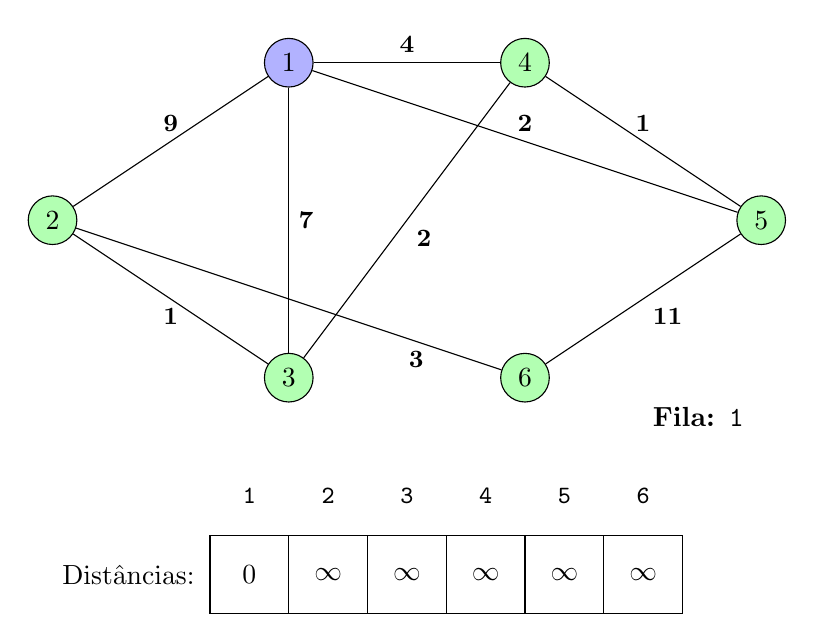
\begin{tikzpicture}
        \node[anchor=west] at (0, 0.5) { Distâncias: };
        \node[anchor=west] at (7.5, 2.5) { \bfseries Fila: \texttt{1} };

        \node[circle, draw, fill=blue!30] (a) at (3, 7) {1};
        \node[circle, draw, fill=green!30] (b) at (0, 5) {2};
        \node[circle, draw, fill=green!30] (c) at (3, 3) {3};
        \node[circle, draw, fill=green!30] (d) at (6, 7) {4};
        \node[circle, draw, fill=green!30] (e) at (9, 5) {5};
        \node[circle, draw, fill=green!30] (f) at (6, 3) {6};

        \draw (2, 0) grid (8, 1);

        \node at (2.5, 0.5) { $0$ };
        \node at (3.5, 0.5) { \textcolor{black}{$\infty$} };
        \node at (4.5, 0.5) { \textcolor{black}{$\infty$} };
        \node at (5.5, 0.5) { \textcolor{black}{$\infty$} };
        \node at (6.5, 0.5) { \textcolor{black}{$\infty$} };
        \node at (7.5, 0.5) { \textcolor{black}{$\infty$} };

        \node at (2.5, 1.5) { \small \texttt{1} };
        \node at (3.5, 1.5) { \small \texttt{2} };
        \node at (4.5, 1.5) { \small \texttt{3} };
        \node at (5.5, 1.5) { \small \texttt{4} };
        \node at (6.5, 1.5) { \small \texttt{5} };
        \node at (7.5, 1.5) { \small \texttt{6} };

        \draw (a) to node[midway,anchor=south] { \small \bfseries 9 } (b);
        \draw (a) to node[midway,anchor=west] { \small \bfseries 7 } (c);
        \draw (a) to node[midway,anchor=south] { \small \bfseries 4 } (d);
        \draw (a) to node[midway,anchor=south] { \small \bfseries 2 } (e);
        \draw (b) to node[midway,anchor=north] { \small \bfseries 1 } (c);
        \draw (b) to node[pos=0.8,anchor=north] { \small \bfseries 3 } (f);
        \draw (c) to node[midway,anchor=north west] { \small \bfseries 2 } (d);
        \draw (d) to node[midway,anchor=south] { \small \bfseries 1 } (e);
        \draw (e) to node[midway,anchor=north west] { \small \bfseries 11 } (f);

    \end{tikzpicture}

\end{frame}


\begin{frame}[fragile]{Visualização do algoritmo SPFA}

    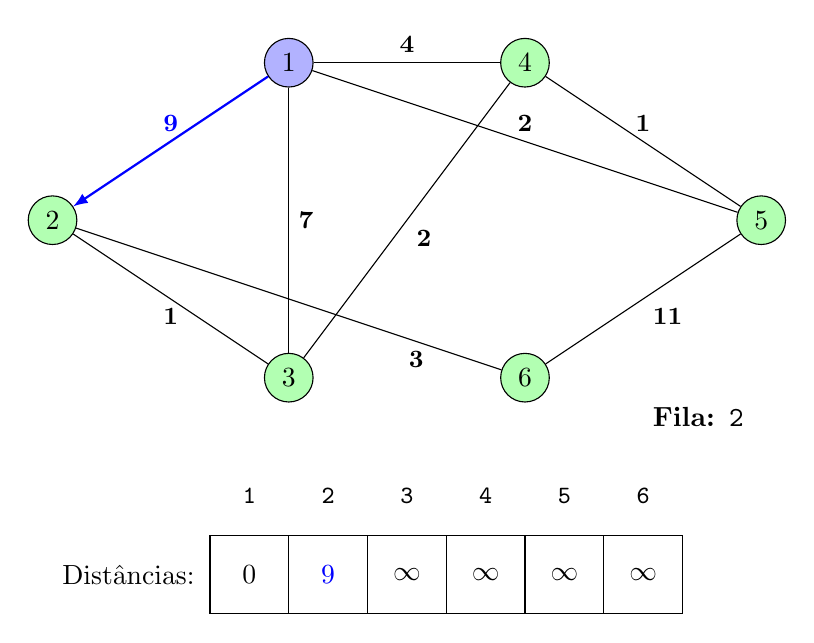
\begin{tikzpicture}
        \node[anchor=west] at (0, 0.5) { Distâncias: };
        \node[anchor=west] at (7.5, 2.5) { \bfseries Fila: \texttt{2} };

        \node[circle, draw, fill=blue!30] (a) at (3, 7) {1};
        \node[circle, draw, fill=green!30] (b) at (0, 5) {2};
        \node[circle, draw, fill=green!30] (c) at (3, 3) {3};
        \node[circle, draw, fill=green!30] (d) at (6, 7) {4};
        \node[circle, draw, fill=green!30] (e) at (9, 5) {5};
        \node[circle, draw, fill=green!30] (f) at (6, 3) {6};

        \draw (2, 0) grid (8, 1);

        \node at (2.5, 0.5) { $0$ };
        \node at (3.5, 0.5) { \textcolor{blue}{$9$} };
        \node at (4.5, 0.5) { \textcolor{black}{$\infty$} };
        \node at (5.5, 0.5) { \textcolor{black}{$\infty$} };
        \node at (6.5, 0.5) { \textcolor{black}{$\infty$} };
        \node at (7.5, 0.5) { \textcolor{black}{$\infty$} };

        \node at (2.5, 1.5) { \small \texttt{1} };
        \node at (3.5, 1.5) { \small \texttt{2} };
        \node at (4.5, 1.5) { \small \texttt{3} };
        \node at (5.5, 1.5) { \small \texttt{4} };
        \node at (6.5, 1.5) { \small \texttt{5} };
        \node at (7.5, 1.5) { \small \texttt{6} };

        %\draw (a) to node[midway,anchor=south] { \small \bfseries 9 } (b);
        \draw[-latex,thick,blue] (a) to node[midway,anchor=south] { \small \bfseries 9 } (b);
        \draw (a) to node[midway,anchor=west] { \small \bfseries 7 } (c);
        \draw (a) to node[midway,anchor=south] { \small \bfseries 4 } (d);
        \draw (a) to node[midway,anchor=south] { \small \bfseries 2 } (e);
        \draw (b) to node[midway,anchor=north] { \small \bfseries 1 } (c);
        \draw (b) to node[pos=0.8,anchor=north] { \small \bfseries 3 } (f);
        \draw (c) to node[midway,anchor=north west] { \small \bfseries 2 } (d);
        \draw (d) to node[midway,anchor=south] { \small \bfseries 1 } (e);
        \draw (e) to node[midway,anchor=north west] { \small \bfseries 11 } (f);

    \end{tikzpicture}

\end{frame}

\begin{frame}[fragile]{Visualização do algoritmo SPFA}

    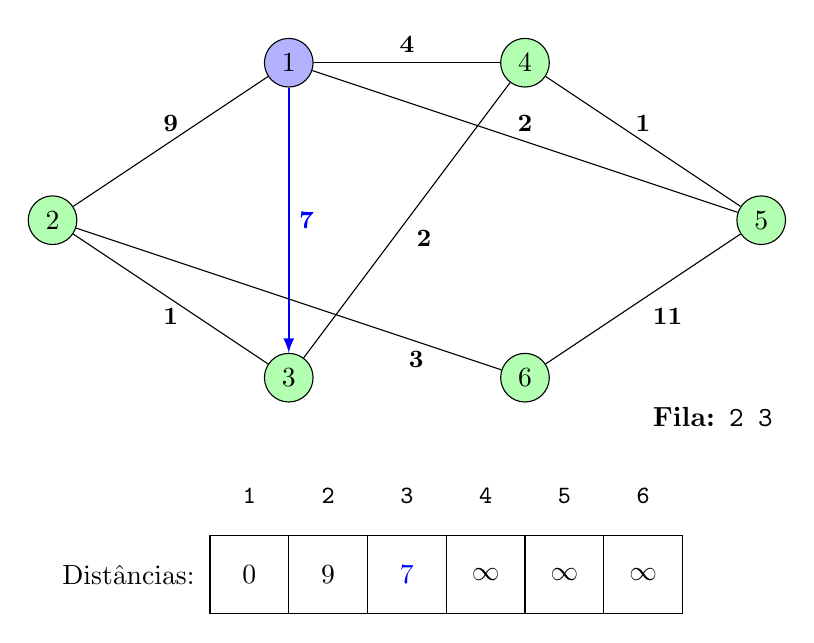
\begin{tikzpicture}
        \node[anchor=west] at (0, 0.5) { Distâncias: };
        \node[anchor=west] at (7.5, 2.5) { \bfseries Fila: \texttt{2 3} };

        \node[circle, draw, fill=blue!30] (a) at (3, 7) {1};
        \node[circle, draw, fill=green!30] (b) at (0, 5) {2};
        \node[circle, draw, fill=green!30] (c) at (3, 3) {3};
        \node[circle, draw, fill=green!30] (d) at (6, 7) {4};
        \node[circle, draw, fill=green!30] (e) at (9, 5) {5};
        \node[circle, draw, fill=green!30] (f) at (6, 3) {6};

        \draw (2, 0) grid (8, 1);

        \node at (2.5, 0.5) { $0$ };
        \node at (3.5, 0.5) { \textcolor{black}{$9$} };
        \node at (4.5, 0.5) { \textcolor{blue}{$7$} };
        \node at (5.5, 0.5) { \textcolor{black}{$\infty$} };
        \node at (6.5, 0.5) { \textcolor{black}{$\infty$} };
        \node at (7.5, 0.5) { \textcolor{black}{$\infty$} };

        \node at (2.5, 1.5) { \small \texttt{1} };
        \node at (3.5, 1.5) { \small \texttt{2} };
        \node at (4.5, 1.5) { \small \texttt{3} };
        \node at (5.5, 1.5) { \small \texttt{4} };
        \node at (6.5, 1.5) { \small \texttt{5} };
        \node at (7.5, 1.5) { \small \texttt{6} };

        \draw (a) to node[midway,anchor=south] { \small \bfseries 9 } (b);
        %\draw (a) to node[midway,anchor=west] { \small \bfseries 7 } (c);
        \draw[-latex,thick,blue] (a) to node[midway,anchor=west] { \small \bfseries 7 } (c);
        \draw (a) to node[midway,anchor=south] { \small \bfseries 4 } (d);
        \draw (a) to node[midway,anchor=south] { \small \bfseries 2 } (e);
        \draw (b) to node[midway,anchor=north] { \small \bfseries 1 } (c);
        \draw (b) to node[pos=0.8,anchor=north] { \small \bfseries 3 } (f);
        \draw (c) to node[midway,anchor=north west] { \small \bfseries 2 } (d);
        \draw (d) to node[midway,anchor=south] { \small \bfseries 1 } (e);
        \draw (e) to node[midway,anchor=north west] { \small \bfseries 11 } (f);

    \end{tikzpicture}

\end{frame}

\begin{frame}[fragile]{Visualização do algoritmo SPFA}

    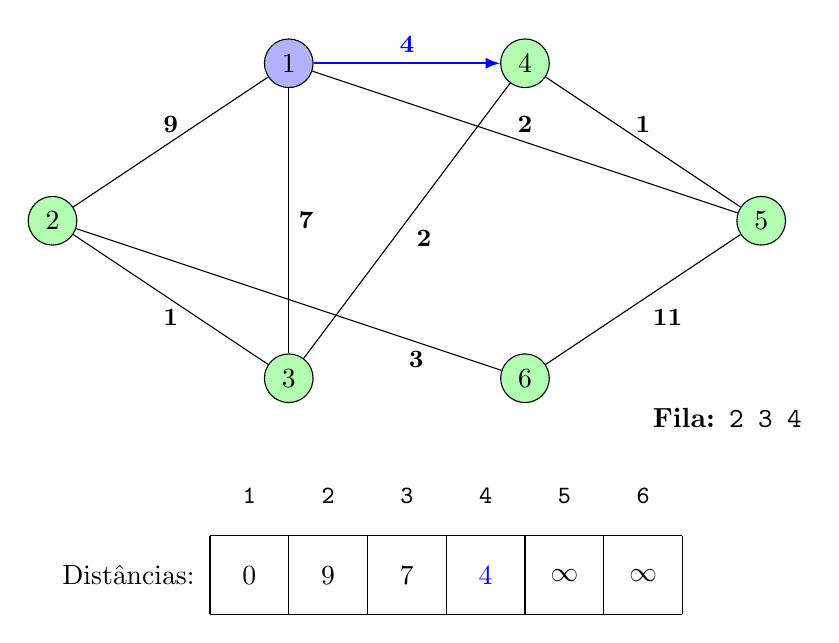
\begin{tikzpicture}
        \node[anchor=west] at (0, 0.5) { Distâncias: };
        \node[anchor=west] at (7.5, 2.5) { \bfseries Fila: \texttt{2 3 4} };

        \node[circle, draw, fill=blue!30] (a) at (3, 7) {1};
        \node[circle, draw, fill=green!30] (b) at (0, 5) {2};
        \node[circle, draw, fill=green!30] (c) at (3, 3) {3};
        \node[circle, draw, fill=green!30] (d) at (6, 7) {4};
        \node[circle, draw, fill=green!30] (e) at (9, 5) {5};
        \node[circle, draw, fill=green!30] (f) at (6, 3) {6};

        \draw (2, 0) grid (8, 1);

        \node at (2.5, 0.5) { $0$ };
        \node at (3.5, 0.5) { \textcolor{black}{$9$} };
        \node at (4.5, 0.5) { \textcolor{black}{$7$} };
        \node at (5.5, 0.5) { \textcolor{blue}{$4$} };
        \node at (6.5, 0.5) { \textcolor{black}{$\infty$} };
        \node at (7.5, 0.5) { \textcolor{black}{$\infty$} };

        \node at (2.5, 1.5) { \small \texttt{1} };
        \node at (3.5, 1.5) { \small \texttt{2} };
        \node at (4.5, 1.5) { \small \texttt{3} };
        \node at (5.5, 1.5) { \small \texttt{4} };
        \node at (6.5, 1.5) { \small \texttt{5} };
        \node at (7.5, 1.5) { \small \texttt{6} };

        \draw (a) to node[midway,anchor=south] { \small \bfseries 9 } (b);
        \draw (a) to node[midway,anchor=west] { \small \bfseries 7 } (c);
        %\draw (a) to node[midway,anchor=south] { \small \bfseries 4 } (d);
        \draw[-latex,thick,blue] (a) to node[midway,anchor=south] { \small \bfseries 4 } (d);
        \draw (a) to node[midway,anchor=south] { \small \bfseries 2 } (e);
        \draw (b) to node[midway,anchor=north] { \small \bfseries 1 } (c);
        \draw (b) to node[pos=0.8,anchor=north] { \small \bfseries 3 } (f);
        \draw (c) to node[midway,anchor=north west] { \small \bfseries 2 } (d);
        \draw (d) to node[midway,anchor=south] { \small \bfseries 1 } (e);
        \draw (e) to node[midway,anchor=north west] { \small \bfseries 11 } (f);

    \end{tikzpicture}

\end{frame}

\begin{frame}[fragile]{Visualização do algoritmo SPFA}

    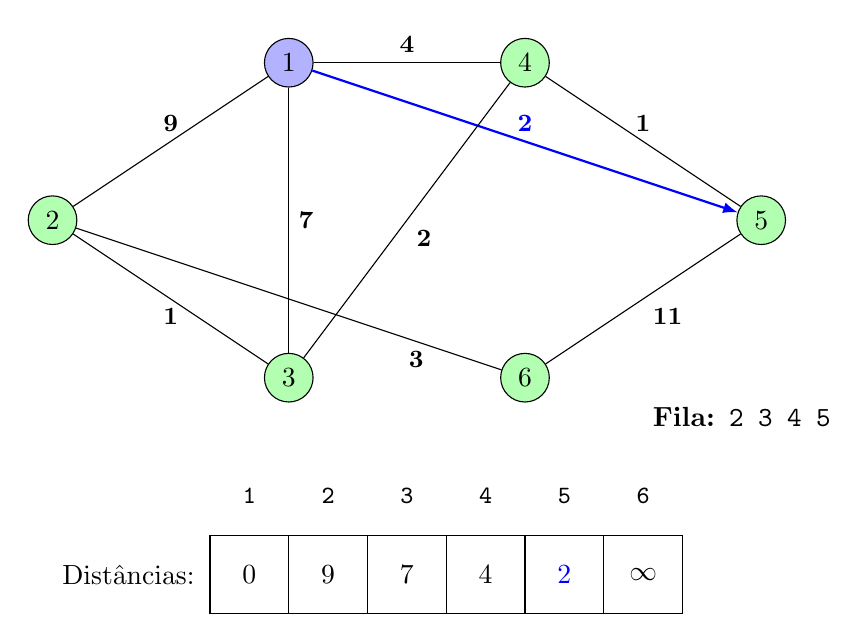
\begin{tikzpicture}
        \node[anchor=west] at (0, 0.5) { Distâncias: };
        \node[anchor=west] at (7.5, 2.5) { \bfseries Fila: \texttt{2 3 4 5} };

        \node[circle, draw, fill=blue!30] (a) at (3, 7) {1};
        \node[circle, draw, fill=green!30] (b) at (0, 5) {2};
        \node[circle, draw, fill=green!30] (c) at (3, 3) {3};
        \node[circle, draw, fill=green!30] (d) at (6, 7) {4};
        \node[circle, draw, fill=green!30] (e) at (9, 5) {5};
        \node[circle, draw, fill=green!30] (f) at (6, 3) {6};

        \draw (2, 0) grid (8, 1);

        \node at (2.5, 0.5) { $0$ };
        \node at (3.5, 0.5) { \textcolor{black}{$9$} };
        \node at (4.5, 0.5) { \textcolor{black}{$7$} };
        \node at (5.5, 0.5) { \textcolor{black}{$4$} };
        \node at (6.5, 0.5) { \textcolor{blue}{$2$} };
        \node at (7.5, 0.5) { \textcolor{black}{$\infty$} };

        \node at (2.5, 1.5) { \small \texttt{1} };
        \node at (3.5, 1.5) { \small \texttt{2} };
        \node at (4.5, 1.5) { \small \texttt{3} };
        \node at (5.5, 1.5) { \small \texttt{4} };
        \node at (6.5, 1.5) { \small \texttt{5} };
        \node at (7.5, 1.5) { \small \texttt{6} };

        \draw (a) to node[midway,anchor=south] { \small \bfseries 9 } (b);
        \draw (a) to node[midway,anchor=west] { \small \bfseries 7 } (c);
        \draw (a) to node[midway,anchor=south] { \small \bfseries 4 } (d);
        %\draw (a) to node[midway,anchor=south] { \small \bfseries 2 } (e);
        \draw[-latex,thick,blue] (a) to node[midway,anchor=south] { \small \bfseries 2 } (e);
        \draw (b) to node[midway,anchor=north] { \small \bfseries 1 } (c);
        \draw (b) to node[pos=0.8,anchor=north] { \small \bfseries 3 } (f);
        \draw (c) to node[midway,anchor=north west] { \small \bfseries 2 } (d);
        \draw (d) to node[midway,anchor=south] { \small \bfseries 1 } (e);
        \draw (e) to node[midway,anchor=north west] { \small \bfseries 11 } (f);

    \end{tikzpicture}

\end{frame}

\begin{frame}[fragile]{Visualização do algoritmo SPFA}

    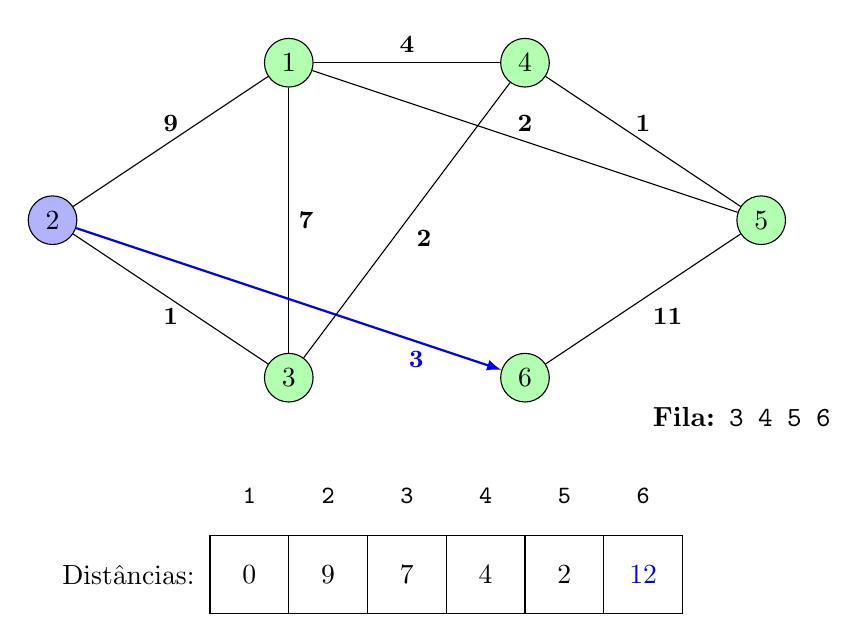
\begin{tikzpicture}
        \node[anchor=west] at (0, 0.5) { Distâncias: };
        \node[anchor=west] at (7.5, 2.5) { \bfseries Fila: \texttt{3 4 5 6} };

        \node[circle, draw, fill=green!30] (a) at (3, 7) {1};
        \node[circle, draw, fill=blue!30] (b) at (0, 5) {2};
        \node[circle, draw, fill=green!30] (c) at (3, 3) {3};
        \node[circle, draw, fill=green!30] (d) at (6, 7) {4};
        \node[circle, draw, fill=green!30] (e) at (9, 5) {5};
        \node[circle, draw, fill=green!30] (f) at (6, 3) {6};

        \draw (2, 0) grid (8, 1);

        \node at (2.5, 0.5) { $0$ };
        \node at (3.5, 0.5) { \textcolor{black}{$9$} };
        \node at (4.5, 0.5) { \textcolor{black}{$7$} };
        \node at (5.5, 0.5) { \textcolor{black}{$4$} };
        \node at (6.5, 0.5) { \textcolor{black}{$2$} };
        \node at (7.5, 0.5) { \textcolor{blue}{$12$} };

        \node at (2.5, 1.5) { \small \texttt{1} };
        \node at (3.5, 1.5) { \small \texttt{2} };
        \node at (4.5, 1.5) { \small \texttt{3} };
        \node at (5.5, 1.5) { \small \texttt{4} };
        \node at (6.5, 1.5) { \small \texttt{5} };
        \node at (7.5, 1.5) { \small \texttt{6} };

        \draw (a) to node[midway,anchor=south] { \small \bfseries 9 } (b);
        \draw (a) to node[midway,anchor=west] { \small \bfseries 7 } (c);
        \draw (a) to node[midway,anchor=south] { \small \bfseries 4 } (d);
        \draw (a) to node[midway,anchor=south] { \small \bfseries 2 } (e);
        \draw (b) to node[midway,anchor=north] { \small \bfseries 1 } (c);
        %\draw (b) to node[pos=0.8,anchor=north] { \small \bfseries 3 } (f);
        \draw[-latex,thick,blue] (b) to node[pos=0.8,anchor=north] { \small \bfseries 3 } (f);
        \draw (c) to node[midway,anchor=north west] { \small \bfseries 2 } (d);
        \draw (d) to node[midway,anchor=south] { \small \bfseries 1 } (e);
        \draw (e) to node[midway,anchor=north west] { \small \bfseries 11 } (f);

    \end{tikzpicture}

\end{frame}


\begin{frame}[fragile]{Visualização do algoritmo SPFA}

    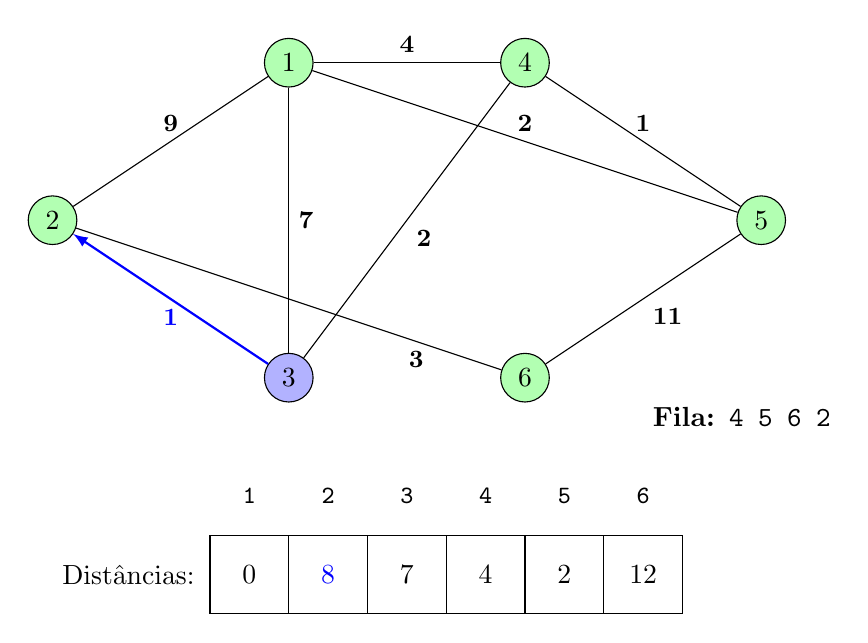
\begin{tikzpicture}
        \node[anchor=west] at (0, 0.5) { Distâncias: };
        \node[anchor=west] at (7.5, 2.5) { \bfseries Fila: \texttt{4 5 6 2} };

        \node[circle, draw, fill=green!30] (a) at (3, 7) {1};
        \node[circle, draw, fill=green!30] (b) at (0, 5) {2};
        \node[circle, draw, fill=blue!30] (c) at (3, 3) {3};
        \node[circle, draw, fill=green!30] (d) at (6, 7) {4};
        \node[circle, draw, fill=green!30] (e) at (9, 5) {5};
        \node[circle, draw, fill=green!30] (f) at (6, 3) {6};

        \draw (2, 0) grid (8, 1);

        \node at (2.5, 0.5) { $0$ };
        \node at (3.5, 0.5) { \textcolor{blue}{$8$} };
        \node at (4.5, 0.5) { \textcolor{black}{$7$} };
        \node at (5.5, 0.5) { \textcolor{black}{$4$} };
        \node at (6.5, 0.5) { \textcolor{black}{$2$} };
        \node at (7.5, 0.5) { \textcolor{black}{$12$} };

        \node at (2.5, 1.5) { \small \texttt{1} };
        \node at (3.5, 1.5) { \small \texttt{2} };
        \node at (4.5, 1.5) { \small \texttt{3} };
        \node at (5.5, 1.5) { \small \texttt{4} };
        \node at (6.5, 1.5) { \small \texttt{5} };
        \node at (7.5, 1.5) { \small \texttt{6} };

        \draw (a) to node[midway,anchor=south] { \small \bfseries 9 } (b);
        \draw (a) to node[midway,anchor=west] { \small \bfseries 7 } (c);
        \draw (a) to node[midway,anchor=south] { \small \bfseries 4 } (d);
        \draw (a) to node[midway,anchor=south] { \small \bfseries 2 } (e);
        %\draw (b) to node[midway,anchor=north] { \small \bfseries 1 } (c);
        \draw[latex-,thick,blue] (b) to node[midway,anchor=north] { \small \bfseries 1 } (c);
        \draw (b) to node[pos=0.8,anchor=north] { \small \bfseries 3 } (f);
        \draw (c) to node[midway,anchor=north west] { \small \bfseries 2 } (d);
        \draw (d) to node[midway,anchor=south] { \small \bfseries 1 } (e);
        \draw (e) to node[midway,anchor=north west] { \small \bfseries 11 } (f);

    \end{tikzpicture}

\end{frame}


\begin{frame}[fragile]{Visualização do algoritmo SPFA}

    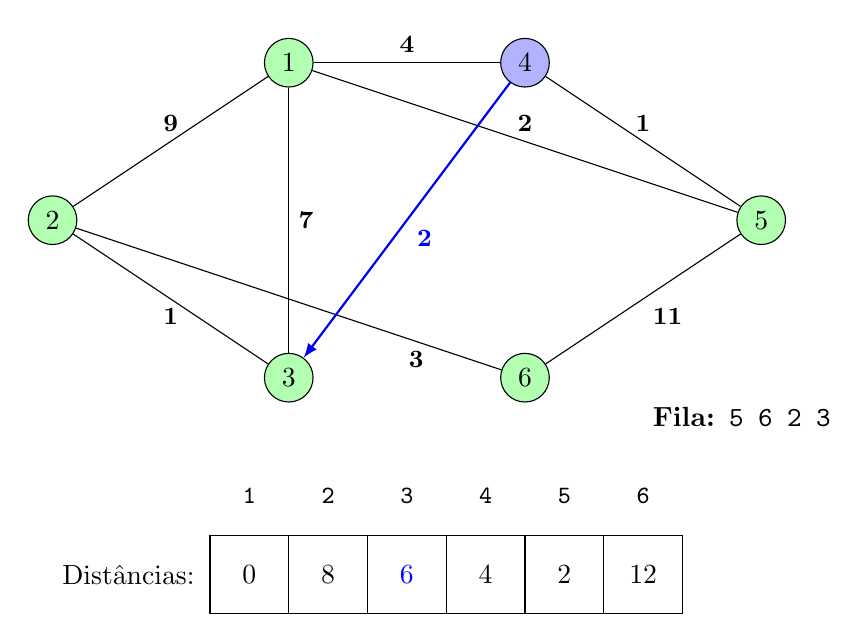
\begin{tikzpicture}
        \node[anchor=west] at (0, 0.5) { Distâncias: };
        \node[anchor=west] at (7.5, 2.5) { \bfseries Fila: \texttt{5 6 2 3} };

        \node[circle, draw, fill=green!30] (a) at (3, 7) {1};
        \node[circle, draw, fill=green!30] (b) at (0, 5) {2};
        \node[circle, draw, fill=green!30] (c) at (3, 3) {3};
        \node[circle, draw, fill=blue!30] (d) at (6, 7) {4};
        \node[circle, draw, fill=green!30] (e) at (9, 5) {5};
        \node[circle, draw, fill=green!30] (f) at (6, 3) {6};

        \draw (2, 0) grid (8, 1);

        \node at (2.5, 0.5) { $0$ };
        \node at (3.5, 0.5) { \textcolor{black}{$8$} };
        \node at (4.5, 0.5) { \textcolor{blue}{$6$} };
        \node at (5.5, 0.5) { \textcolor{black}{$4$} };
        \node at (6.5, 0.5) { \textcolor{black}{$2$} };
        \node at (7.5, 0.5) { \textcolor{black}{$12$} };

        \node at (2.5, 1.5) { \small \texttt{1} };
        \node at (3.5, 1.5) { \small \texttt{2} };
        \node at (4.5, 1.5) { \small \texttt{3} };
        \node at (5.5, 1.5) { \small \texttt{4} };
        \node at (6.5, 1.5) { \small \texttt{5} };
        \node at (7.5, 1.5) { \small \texttt{6} };

        \draw (a) to node[midway,anchor=south] { \small \bfseries 9 } (b);
        \draw (a) to node[midway,anchor=west] { \small \bfseries 7 } (c);
        \draw (a) to node[midway,anchor=south] { \small \bfseries 4 } (d);
        \draw (a) to node[midway,anchor=south] { \small \bfseries 2 } (e);
        \draw (b) to node[midway,anchor=north] { \small \bfseries 1 } (c);
        \draw (b) to node[pos=0.8,anchor=north] { \small \bfseries 3 } (f);
        %\draw (c) to node[midway,anchor=north west] { \small \bfseries 2 } (d);
        \draw[latex-,thick,blue] (c) to node[midway,anchor=north west] { \small \bfseries 2 } (d);
        \draw (d) to node[midway,anchor=south] { \small \bfseries 1 } (e);
        \draw (e) to node[midway,anchor=north west] { \small \bfseries 11 } (f);

    \end{tikzpicture}

\end{frame}

\begin{frame}[fragile]{Visualização do algoritmo SPFA}

    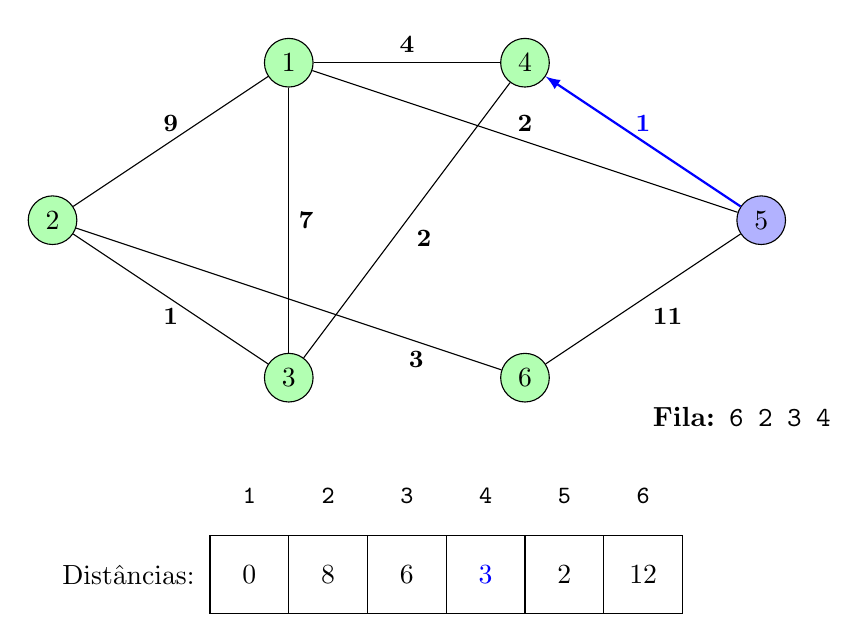
\begin{tikzpicture}
        \node[anchor=west] at (0, 0.5) { Distâncias: };
        \node[anchor=west] at (7.5, 2.5) { \bfseries Fila: \texttt{6 2 3 4} };

        \node[circle, draw, fill=green!30] (a) at (3, 7) {1};
        \node[circle, draw, fill=green!30] (b) at (0, 5) {2};
        \node[circle, draw, fill=green!30] (c) at (3, 3) {3};
        \node[circle, draw, fill=green!30] (d) at (6, 7) {4};
        \node[circle, draw, fill=blue!30] (e) at (9, 5) {5};
        \node[circle, draw, fill=green!30] (f) at (6, 3) {6};

        \draw (2, 0) grid (8, 1);

        \node at (2.5, 0.5) { $0$ };
        \node at (3.5, 0.5) { \textcolor{black}{$8$} };
        \node at (4.5, 0.5) { \textcolor{black}{$6$} };
        \node at (5.5, 0.5) { \textcolor{blue}{$3$} };
        \node at (6.5, 0.5) { \textcolor{black}{$2$} };
        \node at (7.5, 0.5) { \textcolor{black}{$12$} };

        \node at (2.5, 1.5) { \small \texttt{1} };
        \node at (3.5, 1.5) { \small \texttt{2} };
        \node at (4.5, 1.5) { \small \texttt{3} };
        \node at (5.5, 1.5) { \small \texttt{4} };
        \node at (6.5, 1.5) { \small \texttt{5} };
        \node at (7.5, 1.5) { \small \texttt{6} };

        \draw (a) to node[midway,anchor=south] { \small \bfseries 9 } (b);
        \draw (a) to node[midway,anchor=west] { \small \bfseries 7 } (c);
        \draw (a) to node[midway,anchor=south] { \small \bfseries 4 } (d);
        \draw (a) to node[midway,anchor=south] { \small \bfseries 2 } (e);
        \draw (b) to node[midway,anchor=north] { \small \bfseries 1 } (c);
        \draw (b) to node[pos=0.8,anchor=north] { \small \bfseries 3 } (f);
        \draw (c) to node[midway,anchor=north west] { \small \bfseries 2 } (d);
        %\draw (d) to node[midway,anchor=south] { \small \bfseries 1 } (e);
        \draw[latex-,thick,blue] (d) to node[midway,anchor=south] { \small \bfseries 1 } (e);
        \draw (e) to node[midway,anchor=north west] { \small \bfseries 11 } (f);

    \end{tikzpicture}

\end{frame}

\begin{frame}[fragile]{Visualização do algoritmo SPFA}

    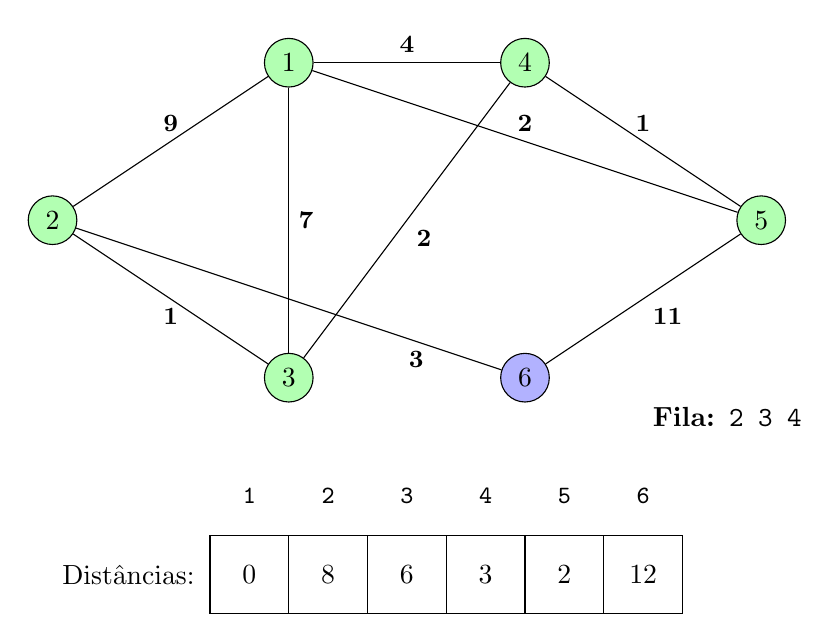
\begin{tikzpicture}
        \node[anchor=west] at (0, 0.5) { Distâncias: };
        \node[anchor=west] at (7.5, 2.5) { \bfseries Fila: \texttt{2 3 4} };

        \node[circle, draw, fill=green!30] (a) at (3, 7) {1};
        \node[circle, draw, fill=green!30] (b) at (0, 5) {2};
        \node[circle, draw, fill=green!30] (c) at (3, 3) {3};
        \node[circle, draw, fill=green!30] (d) at (6, 7) {4};
        \node[circle, draw, fill=green!30] (e) at (9, 5) {5};
        \node[circle, draw, fill=blue!30] (f) at (6, 3) {6};

        \draw (2, 0) grid (8, 1);

        \node at (2.5, 0.5) { $0$ };
        \node at (3.5, 0.5) { \textcolor{black}{$8$} };
        \node at (4.5, 0.5) { \textcolor{black}{$6$} };
        \node at (5.5, 0.5) { \textcolor{black}{$3$} };
        \node at (6.5, 0.5) { \textcolor{black}{$2$} };
        \node at (7.5, 0.5) { \textcolor{black}{$12$} };

        \node at (2.5, 1.5) { \small \texttt{1} };
        \node at (3.5, 1.5) { \small \texttt{2} };
        \node at (4.5, 1.5) { \small \texttt{3} };
        \node at (5.5, 1.5) { \small \texttt{4} };
        \node at (6.5, 1.5) { \small \texttt{5} };
        \node at (7.5, 1.5) { \small \texttt{6} };

        \draw (a) to node[midway,anchor=south] { \small \bfseries 9 } (b);
        \draw (a) to node[midway,anchor=west] { \small \bfseries 7 } (c);
        \draw (a) to node[midway,anchor=south] { \small \bfseries 4 } (d);
        \draw (a) to node[midway,anchor=south] { \small \bfseries 2 } (e);
        \draw (b) to node[midway,anchor=north] { \small \bfseries 1 } (c);
        \draw (b) to node[pos=0.8,anchor=north] { \small \bfseries 3 } (f);
        \draw (c) to node[midway,anchor=north west] { \small \bfseries 2 } (d);
        \draw (d) to node[midway,anchor=south] { \small \bfseries 1 } (e);
        \draw (e) to node[midway,anchor=north west] { \small \bfseries 11 } (f);

    \end{tikzpicture}

\end{frame}


\begin{frame}[fragile]{Visualização do algoritmo SPFA}

    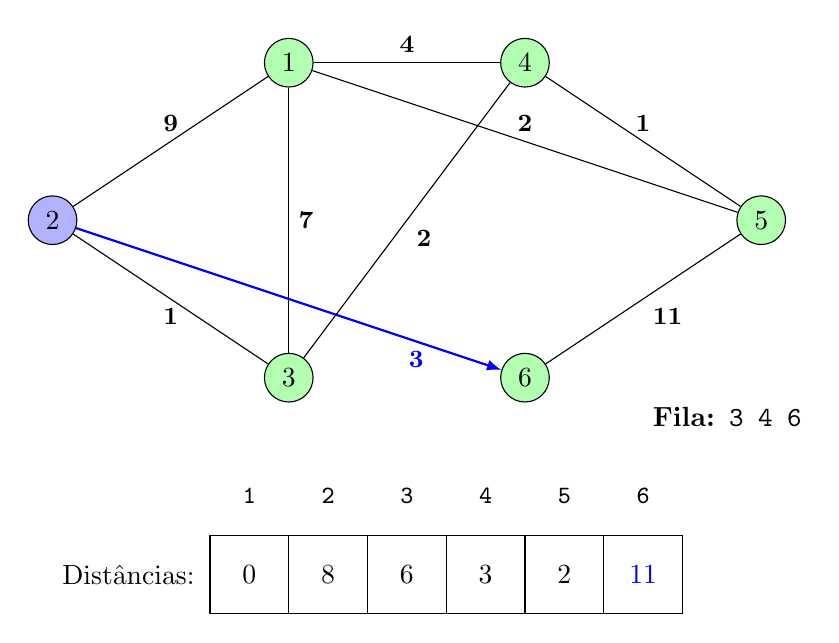
\begin{tikzpicture}
        \node[anchor=west] at (0, 0.5) { Distâncias: };
        \node[anchor=west] at (7.5, 2.5) { \bfseries Fila: \texttt{3 4 6} };

        \node[circle, draw, fill=green!30] (a) at (3, 7) {1};
        \node[circle, draw, fill=blue!30] (b) at (0, 5) {2};
        \node[circle, draw, fill=green!30] (c) at (3, 3) {3};
        \node[circle, draw, fill=green!30] (d) at (6, 7) {4};
        \node[circle, draw, fill=green!30] (e) at (9, 5) {5};
        \node[circle, draw, fill=green!30] (f) at (6, 3) {6};

        \draw (2, 0) grid (8, 1);

        \node at (2.5, 0.5) { $0$ };
        \node at (3.5, 0.5) { \textcolor{black}{$8$} };
        \node at (4.5, 0.5) { \textcolor{black}{$6$} };
        \node at (5.5, 0.5) { \textcolor{black}{$3$} };
        \node at (6.5, 0.5) { \textcolor{black}{$2$} };
        \node at (7.5, 0.5) { \textcolor{blue}{$11$} };

        \node at (2.5, 1.5) { \small \texttt{1} };
        \node at (3.5, 1.5) { \small \texttt{2} };
        \node at (4.5, 1.5) { \small \texttt{3} };
        \node at (5.5, 1.5) { \small \texttt{4} };
        \node at (6.5, 1.5) { \small \texttt{5} };
        \node at (7.5, 1.5) { \small \texttt{6} };

        \draw (a) to node[midway,anchor=south] { \small \bfseries 9 } (b);
        \draw (a) to node[midway,anchor=west] { \small \bfseries 7 } (c);
        \draw (a) to node[midway,anchor=south] { \small \bfseries 4 } (d);
        \draw (a) to node[midway,anchor=south] { \small \bfseries 2 } (e);
        \draw (b) to node[midway,anchor=north] { \small \bfseries 1 } (c);
        %\draw (b) to node[pos=0.8,anchor=north] { \small \bfseries 3 } (f);
        \draw[-latex,thick,blue] (b) to node[pos=0.8,anchor=north] { \small \bfseries 3 } (f);
        \draw (c) to node[midway,anchor=north west] { \small \bfseries 2 } (d);
        \draw (d) to node[midway,anchor=south] { \small \bfseries 1 } (e);
        \draw (e) to node[midway,anchor=north west] { \small \bfseries 11 } (f);

    \end{tikzpicture}

\end{frame}

\begin{frame}[fragile]{Visualização do algoritmo SPFA}

    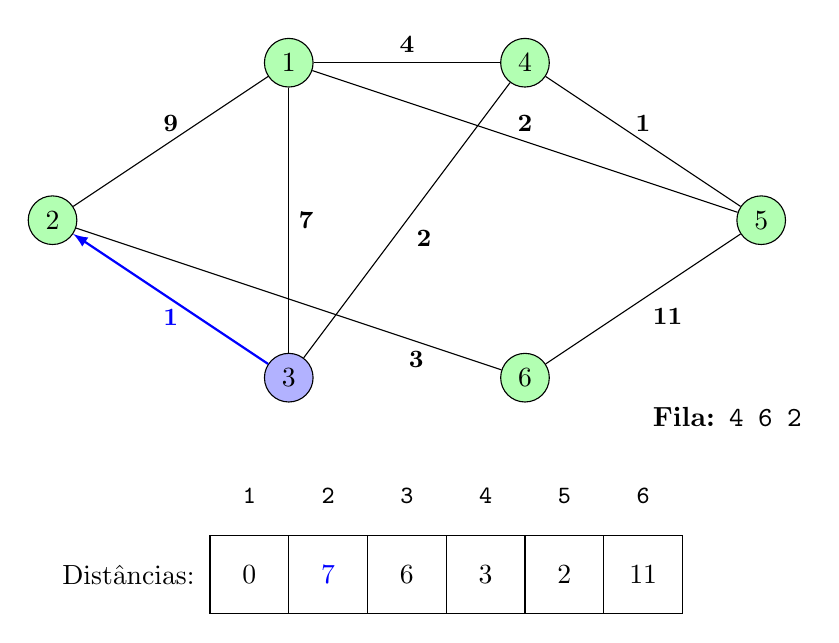
\begin{tikzpicture}
        \node[anchor=west] at (0, 0.5) { Distâncias: };
        \node[anchor=west] at (7.5, 2.5) { \bfseries Fila: \texttt{4 6 2} };

        \node[circle, draw, fill=green!30] (a) at (3, 7) {1};
        \node[circle, draw, fill=green!30] (b) at (0, 5) {2};
        \node[circle, draw, fill=blue!30] (c) at (3, 3) {3};
        \node[circle, draw, fill=green!30] (d) at (6, 7) {4};
        \node[circle, draw, fill=green!30] (e) at (9, 5) {5};
        \node[circle, draw, fill=green!30] (f) at (6, 3) {6};

        \draw (2, 0) grid (8, 1);

        \node at (2.5, 0.5) { $0$ };
        \node at (3.5, 0.5) { \textcolor{blue}{$7$} };
        \node at (4.5, 0.5) { \textcolor{black}{$6$} };
        \node at (5.5, 0.5) { \textcolor{black}{$3$} };
        \node at (6.5, 0.5) { \textcolor{black}{$2$} };
        \node at (7.5, 0.5) { \textcolor{black}{$11$} };

        \node at (2.5, 1.5) { \small \texttt{1} };
        \node at (3.5, 1.5) { \small \texttt{2} };
        \node at (4.5, 1.5) { \small \texttt{3} };
        \node at (5.5, 1.5) { \small \texttt{4} };
        \node at (6.5, 1.5) { \small \texttt{5} };
        \node at (7.5, 1.5) { \small \texttt{6} };

        \draw (a) to node[midway,anchor=south] { \small \bfseries 9 } (b);
        \draw (a) to node[midway,anchor=west] { \small \bfseries 7 } (c);
        \draw (a) to node[midway,anchor=south] { \small \bfseries 4 } (d);
        \draw (a) to node[midway,anchor=south] { \small \bfseries 2 } (e);
        %\draw (b) to node[midway,anchor=north] { \small \bfseries 1 } (c);
        \draw[latex-,thick,blue] (b) to node[midway,anchor=north] { \small \bfseries 1 } (c);
        \draw (b) to node[pos=0.8,anchor=north] { \small \bfseries 3 } (f);
        \draw (c) to node[midway,anchor=north west] { \small \bfseries 2 } (d);
        \draw (d) to node[midway,anchor=south] { \small \bfseries 1 } (e);
        \draw (e) to node[midway,anchor=north west] { \small \bfseries 11 } (f);

    \end{tikzpicture}

\end{frame}

\begin{frame}[fragile]{Visualização do algoritmo SPFA}

    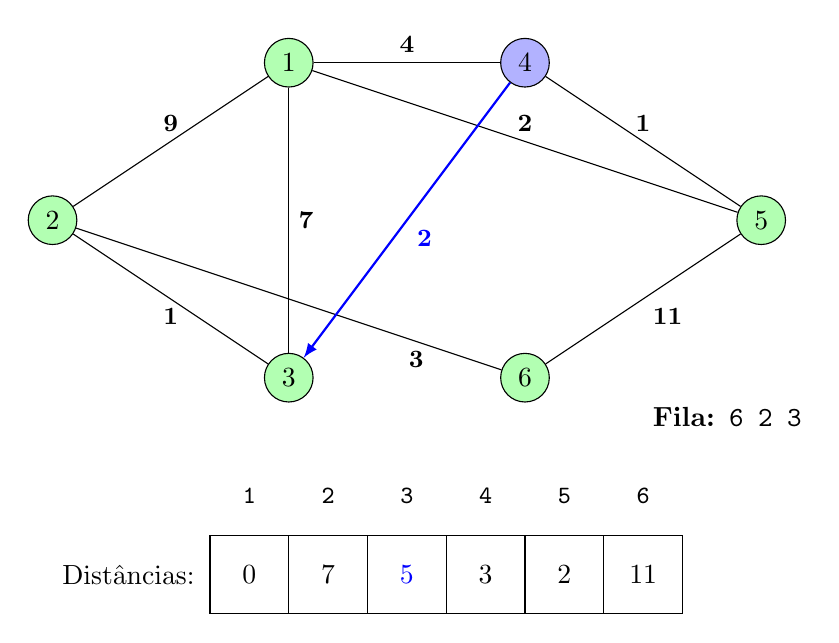
\begin{tikzpicture}
        \node[anchor=west] at (0, 0.5) { Distâncias: };
        \node[anchor=west] at (7.5, 2.5) { \bfseries Fila: \texttt{6 2 3} };

        \node[circle, draw, fill=green!30] (a) at (3, 7) {1};
        \node[circle, draw, fill=green!30] (b) at (0, 5) {2};
        \node[circle, draw, fill=green!30] (c) at (3, 3) {3};
        \node[circle, draw, fill=blue!30] (d) at (6, 7) {4};
        \node[circle, draw, fill=green!30] (e) at (9, 5) {5};
        \node[circle, draw, fill=green!30] (f) at (6, 3) {6};

        \draw (2, 0) grid (8, 1);

        \node at (2.5, 0.5) { $0$ };
        \node at (3.5, 0.5) { \textcolor{black}{$7$} };
        \node at (4.5, 0.5) { \textcolor{blue}{$5$} };
        \node at (5.5, 0.5) { \textcolor{black}{$3$} };
        \node at (6.5, 0.5) { \textcolor{black}{$2$} };
        \node at (7.5, 0.5) { \textcolor{black}{$11$} };

        \node at (2.5, 1.5) { \small \texttt{1} };
        \node at (3.5, 1.5) { \small \texttt{2} };
        \node at (4.5, 1.5) { \small \texttt{3} };
        \node at (5.5, 1.5) { \small \texttt{4} };
        \node at (6.5, 1.5) { \small \texttt{5} };
        \node at (7.5, 1.5) { \small \texttt{6} };

        \draw (a) to node[midway,anchor=south] { \small \bfseries 9 } (b);
        \draw (a) to node[midway,anchor=west] { \small \bfseries 7 } (c);
        \draw (a) to node[midway,anchor=south] { \small \bfseries 4 } (d);
        \draw (a) to node[midway,anchor=south] { \small \bfseries 2 } (e);
        \draw (b) to node[midway,anchor=north] { \small \bfseries 1 } (c);
        \draw (b) to node[pos=0.8,anchor=north] { \small \bfseries 3 } (f);
        %\draw (c) to node[midway,anchor=north west] { \small \bfseries 2 } (d);
        \draw[latex-,thick,blue] (c) to node[midway,anchor=north west] { \small \bfseries 2 } (d);
        \draw (d) to node[midway,anchor=south] { \small \bfseries 1 } (e);
        \draw (e) to node[midway,anchor=north west] { \small \bfseries 11 } (f);

    \end{tikzpicture}

\end{frame}

\begin{frame}[fragile]{Visualização do algoritmo SPFA}

    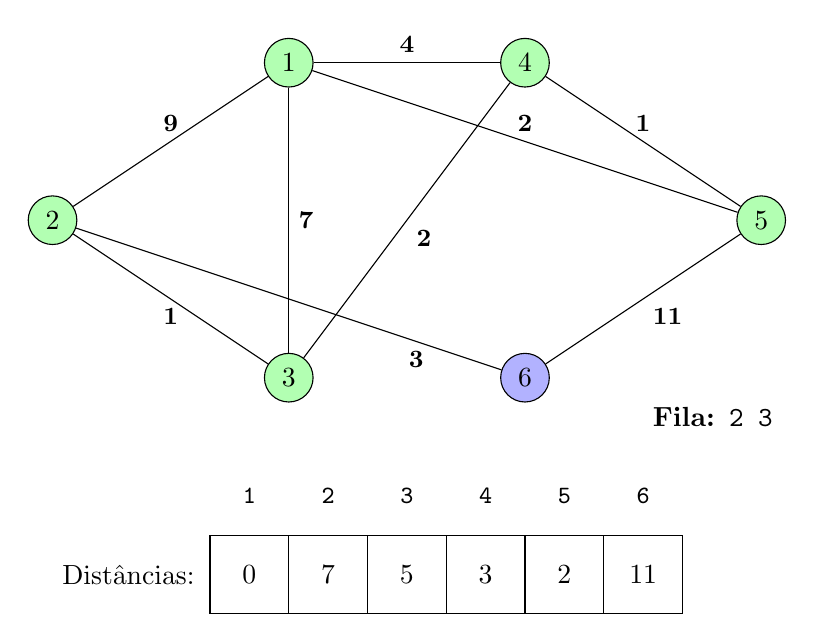
\begin{tikzpicture}
        \node[anchor=west] at (0, 0.5) { Distâncias: };
        \node[anchor=west] at (7.5, 2.5) { \bfseries Fila: \texttt{2 3} };

        \node[circle, draw, fill=green!30] (a) at (3, 7) {1};
        \node[circle, draw, fill=green!30] (b) at (0, 5) {2};
        \node[circle, draw, fill=green!30] (c) at (3, 3) {3};
        \node[circle, draw, fill=green!30] (d) at (6, 7) {4};
        \node[circle, draw, fill=green!30] (e) at (9, 5) {5};
        \node[circle, draw, fill=blue!30] (f) at (6, 3) {6};

        \draw (2, 0) grid (8, 1);

        \node at (2.5, 0.5) { $0$ };
        \node at (3.5, 0.5) { \textcolor{black}{$7$} };
        \node at (4.5, 0.5) { \textcolor{black}{$5$} };
        \node at (5.5, 0.5) { \textcolor{black}{$3$} };
        \node at (6.5, 0.5) { \textcolor{black}{$2$} };
        \node at (7.5, 0.5) { \textcolor{black}{$11$} };

        \node at (2.5, 1.5) { \small \texttt{1} };
        \node at (3.5, 1.5) { \small \texttt{2} };
        \node at (4.5, 1.5) { \small \texttt{3} };
        \node at (5.5, 1.5) { \small \texttt{4} };
        \node at (6.5, 1.5) { \small \texttt{5} };
        \node at (7.5, 1.5) { \small \texttt{6} };

        \draw (a) to node[midway,anchor=south] { \small \bfseries 9 } (b);
        \draw (a) to node[midway,anchor=west] { \small \bfseries 7 } (c);
        \draw (a) to node[midway,anchor=south] { \small \bfseries 4 } (d);
        \draw (a) to node[midway,anchor=south] { \small \bfseries 2 } (e);
        \draw (b) to node[midway,anchor=north] { \small \bfseries 1 } (c);
        \draw (b) to node[pos=0.8,anchor=north] { \small \bfseries 3 } (f);
        \draw (c) to node[midway,anchor=north west] { \small \bfseries 2 } (d);
        \draw (d) to node[midway,anchor=south] { \small \bfseries 1 } (e);
        \draw (e) to node[midway,anchor=north west] { \small \bfseries 11 } (f);

    \end{tikzpicture}

\end{frame}

\begin{frame}[fragile]{Visualização do algoritmo SPFA}

    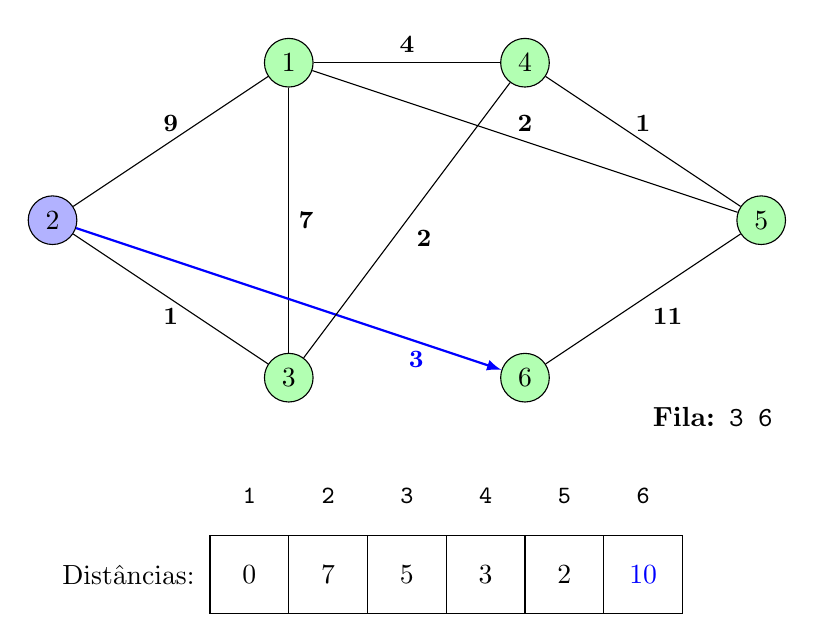
\begin{tikzpicture}
        \node[anchor=west] at (0, 0.5) { Distâncias: };
        \node[anchor=west] at (7.5, 2.5) { \bfseries Fila: \texttt{3 6} };

        \node[circle, draw, fill=green!30] (a) at (3, 7) {1};
        \node[circle, draw, fill=blue!30] (b) at (0, 5) {2};
        \node[circle, draw, fill=green!30] (c) at (3, 3) {3};
        \node[circle, draw, fill=green!30] (d) at (6, 7) {4};
        \node[circle, draw, fill=green!30] (e) at (9, 5) {5};
        \node[circle, draw, fill=green!30] (f) at (6, 3) {6};

        \draw (2, 0) grid (8, 1);

        \node at (2.5, 0.5) { $0$ };
        \node at (3.5, 0.5) { \textcolor{black}{$7$} };
        \node at (4.5, 0.5) { \textcolor{black}{$5$} };
        \node at (5.5, 0.5) { \textcolor{black}{$3$} };
        \node at (6.5, 0.5) { \textcolor{black}{$2$} };
        \node at (7.5, 0.5) { \textcolor{blue}{$10$} };

        \node at (2.5, 1.5) { \small \texttt{1} };
        \node at (3.5, 1.5) { \small \texttt{2} };
        \node at (4.5, 1.5) { \small \texttt{3} };
        \node at (5.5, 1.5) { \small \texttt{4} };
        \node at (6.5, 1.5) { \small \texttt{5} };
        \node at (7.5, 1.5) { \small \texttt{6} };

        \draw (a) to node[midway,anchor=south] { \small \bfseries 9 } (b);
        \draw (a) to node[midway,anchor=west] { \small \bfseries 7 } (c);
        \draw (a) to node[midway,anchor=south] { \small \bfseries 4 } (d);
        \draw (a) to node[midway,anchor=south] { \small \bfseries 2 } (e);
        \draw (b) to node[midway,anchor=north] { \small \bfseries 1 } (c);
        %\draw (b) to node[pos=0.8,anchor=north] { \small \bfseries 3 } (f);
        \draw[-latex,thick,blue] (b) to node[pos=0.8,anchor=north] { \small \bfseries 3 } (f);
        \draw (c) to node[midway,anchor=north west] { \small \bfseries 2 } (d);
        \draw (d) to node[midway,anchor=south] { \small \bfseries 1 } (e);
        \draw (e) to node[midway,anchor=north west] { \small \bfseries 11 } (f);

    \end{tikzpicture}

\end{frame}

\begin{frame}[fragile]{Visualização do algoritmo SPFA}

    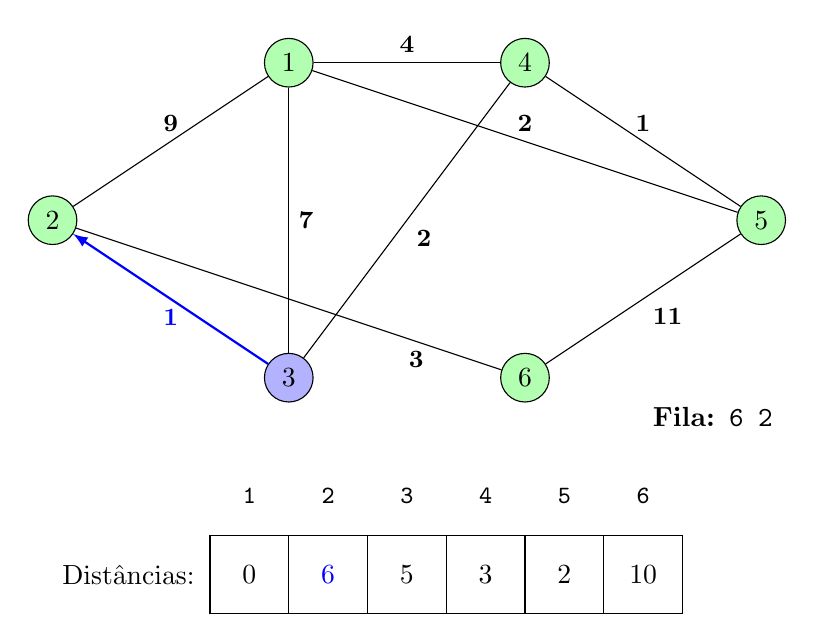
\begin{tikzpicture}
        \node[anchor=west] at (0, 0.5) { Distâncias: };
        \node[anchor=west] at (7.5, 2.5) { \bfseries Fila: \texttt{6 2} };

        \node[circle, draw, fill=green!30] (a) at (3, 7) {1};
        \node[circle, draw, fill=green!30] (b) at (0, 5) {2};
        \node[circle, draw, fill=blue!30] (c) at (3, 3) {3};
        \node[circle, draw, fill=green!30] (d) at (6, 7) {4};
        \node[circle, draw, fill=green!30] (e) at (9, 5) {5};
        \node[circle, draw, fill=green!30] (f) at (6, 3) {6};

        \draw (2, 0) grid (8, 1);

        \node at (2.5, 0.5) { $0$ };
        \node at (3.5, 0.5) { \textcolor{blue}{$6$} };
        \node at (4.5, 0.5) { \textcolor{black}{$5$} };
        \node at (5.5, 0.5) { \textcolor{black}{$3$} };
        \node at (6.5, 0.5) { \textcolor{black}{$2$} };
        \node at (7.5, 0.5) { \textcolor{black}{$10$} };

        \node at (2.5, 1.5) { \small \texttt{1} };
        \node at (3.5, 1.5) { \small \texttt{2} };
        \node at (4.5, 1.5) { \small \texttt{3} };
        \node at (5.5, 1.5) { \small \texttt{4} };
        \node at (6.5, 1.5) { \small \texttt{5} };
        \node at (7.5, 1.5) { \small \texttt{6} };

        \draw (a) to node[midway,anchor=south] { \small \bfseries 9 } (b);
        \draw (a) to node[midway,anchor=west] { \small \bfseries 7 } (c);
        \draw (a) to node[midway,anchor=south] { \small \bfseries 4 } (d);
        \draw (a) to node[midway,anchor=south] { \small \bfseries 2 } (e);
        %\draw (b) to node[midway,anchor=north] { \small \bfseries 1 } (c);
        \draw[latex-,thick,blue] (b) to node[midway,anchor=north] { \small \bfseries 1 } (c);
        \draw (b) to node[pos=0.8,anchor=north] { \small \bfseries 3 } (f);
        \draw (c) to node[midway,anchor=north west] { \small \bfseries 2 } (d);
        \draw (d) to node[midway,anchor=south] { \small \bfseries 1 } (e);
        \draw (e) to node[midway,anchor=north west] { \small \bfseries 11 } (f);

    \end{tikzpicture}

\end{frame}

\begin{frame}[fragile]{Visualização do algoritmo SPFA}

    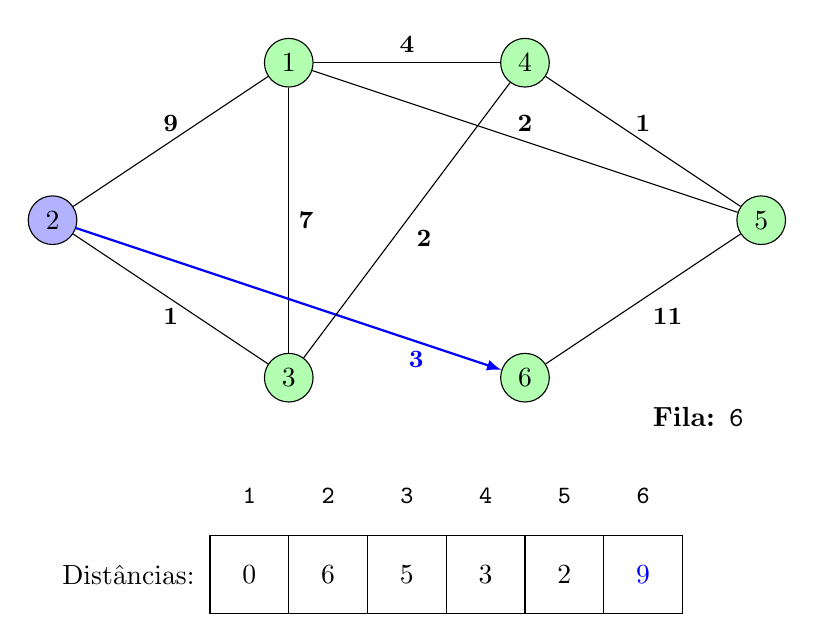
\begin{tikzpicture}
        \node[anchor=west] at (0, 0.5) { Distâncias: };
        \node[anchor=west] at (7.5, 2.5) { \bfseries Fila: \texttt{6} };

        \node[circle, draw, fill=green!30] (a) at (3, 7) {1};
        \node[circle, draw, fill=blue!30] (b) at (0, 5) {2};
        \node[circle, draw, fill=green!30] (c) at (3, 3) {3};
        \node[circle, draw, fill=green!30] (d) at (6, 7) {4};
        \node[circle, draw, fill=green!30] (e) at (9, 5) {5};
        \node[circle, draw, fill=green!30] (f) at (6, 3) {6};

        \draw (2, 0) grid (8, 1);

        \node at (2.5, 0.5) { $0$ };
        \node at (3.5, 0.5) { \textcolor{black}{$6$} };
        \node at (4.5, 0.5) { \textcolor{black}{$5$} };
        \node at (5.5, 0.5) { \textcolor{black}{$3$} };
        \node at (6.5, 0.5) { \textcolor{black}{$2$} };
        \node at (7.5, 0.5) { \textcolor{blue}{$9$} };

        \node at (2.5, 1.5) { \small \texttt{1} };
        \node at (3.5, 1.5) { \small \texttt{2} };
        \node at (4.5, 1.5) { \small \texttt{3} };
        \node at (5.5, 1.5) { \small \texttt{4} };
        \node at (6.5, 1.5) { \small \texttt{5} };
        \node at (7.5, 1.5) { \small \texttt{6} };

        \draw (a) to node[midway,anchor=south] { \small \bfseries 9 } (b);
        \draw (a) to node[midway,anchor=west] { \small \bfseries 7 } (c);
        \draw (a) to node[midway,anchor=south] { \small \bfseries 4 } (d);
        \draw (a) to node[midway,anchor=south] { \small \bfseries 2 } (e);
        \draw (b) to node[midway,anchor=north] { \small \bfseries 1 } (c);
        %\draw (b) to node[pos=0.8,anchor=north] { \small \bfseries 3 } (f);
        \draw[-latex,thick,blue] (b) to node[pos=0.8,anchor=north] { \small \bfseries 3 } (f);
        \draw (c) to node[midway,anchor=north west] { \small \bfseries 2 } (d);
        \draw (d) to node[midway,anchor=south] { \small \bfseries 1 } (e);
        \draw (e) to node[midway,anchor=north west] { \small \bfseries 11 } (f);

    \end{tikzpicture}

\end{frame}

\begin{frame}[fragile]{Visualização do algoritmo SPFA}

    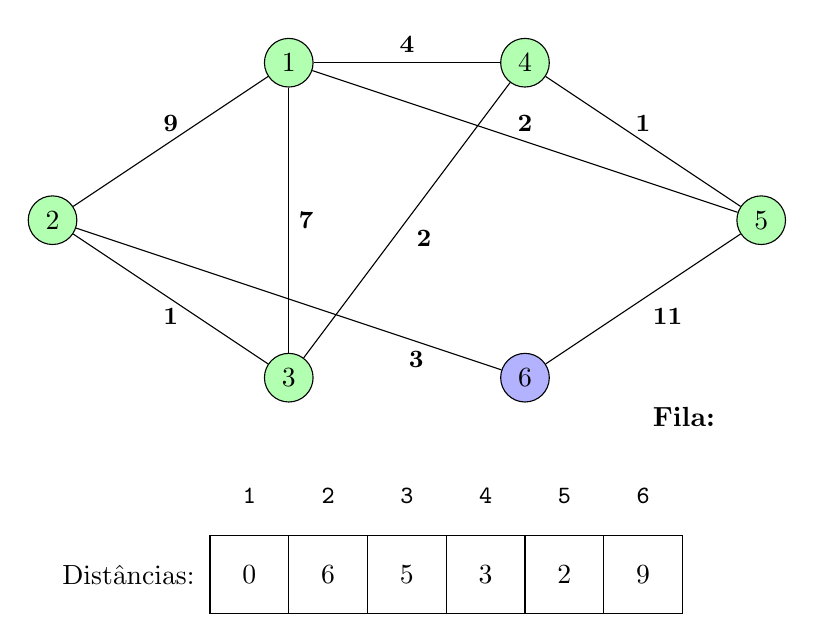
\begin{tikzpicture}
        \node[anchor=west] at (0, 0.5) { Distâncias: };
        \node[anchor=west] at (7.5, 2.5) { \bfseries Fila: \texttt{} };

        \node[circle, draw, fill=green!30] (a) at (3, 7) {1};
        \node[circle, draw, fill=green!30] (b) at (0, 5) {2};
        \node[circle, draw, fill=green!30] (c) at (3, 3) {3};
        \node[circle, draw, fill=green!30] (d) at (6, 7) {4};
        \node[circle, draw, fill=green!30] (e) at (9, 5) {5};
        \node[circle, draw, fill=blue!30] (f) at (6, 3) {6};

        \draw (2, 0) grid (8, 1);

        \node at (2.5, 0.5) { $0$ };
        \node at (3.5, 0.5) { \textcolor{black}{$6$} };
        \node at (4.5, 0.5) { \textcolor{black}{$5$} };
        \node at (5.5, 0.5) { \textcolor{black}{$3$} };
        \node at (6.5, 0.5) { \textcolor{black}{$2$} };
        \node at (7.5, 0.5) { \textcolor{black}{$9$} };

        \node at (2.5, 1.5) { \small \texttt{1} };
        \node at (3.5, 1.5) { \small \texttt{2} };
        \node at (4.5, 1.5) { \small \texttt{3} };
        \node at (5.5, 1.5) { \small \texttt{4} };
        \node at (6.5, 1.5) { \small \texttt{5} };
        \node at (7.5, 1.5) { \small \texttt{6} };

        \draw (a) to node[midway,anchor=south] { \small \bfseries 9 } (b);
        \draw (a) to node[midway,anchor=west] { \small \bfseries 7 } (c);
        \draw (a) to node[midway,anchor=south] { \small \bfseries 4 } (d);
        \draw (a) to node[midway,anchor=south] { \small \bfseries 2 } (e);
        \draw (b) to node[midway,anchor=north] { \small \bfseries 1 } (c);
        \draw (b) to node[pos=0.8,anchor=north] { \small \bfseries 3 } (f);
        \draw (c) to node[midway,anchor=north west] { \small \bfseries 2 } (d);
        \draw (d) to node[midway,anchor=south] { \small \bfseries 1 } (e);
        \draw (e) to node[midway,anchor=north west] { \small \bfseries 11 } (f);

    \end{tikzpicture}

\end{frame}

\begin{frame}[fragile]{Implementação do SPFA em C++}
    \inputsnippet{c++}{1}{21}{spfa.cpp}
\end{frame}

\begin{frame}[fragile]{Implementação do SPFA em C++}
    \inputsnippet{c++}{23}{43}{spfa.cpp}
\end{frame}

\begin{frame}[fragile]{Implementação do SPFA em C++}
    \inputsnippet{c++}{45}{65}{spfa.cpp}
\end{frame}

\begin{frame}[fragile]{SPFA e ciclos negativos}

    \begin{itemize}
        \item A presença de ciclos negativos pode levar o SPFA a um laço infinito, pois a 
            fila nunca ficaria vazia neste caso

        \item Para evitar tal situação, é preciso manter um registro do número de vezes que 
            um nó entrou na fila

        \item Se um mesmo nó tiver entrado $V$ vezes na fila, o grafo tem um ciclo negativo

        \item Com este cuidado adicional, a implementação do SPFA é mais longa do que a do
            algoritmo de Bellman-Ford, mas produz um tempo de execução menor

        \item Para grafos sem a presença de arestas negativas, contudo, há um algoritmo 
            mais eficiente para o mesmo problema: o algoritmo de Djikstra
    \end{itemize}

\end{frame}


